\section{Setup of Rocrail}
t.b.d.

\subsection{Rocrail Controller Settings}

Maak twee controllers, 1 voor can, en 1 voor S88N. screenshots van beide controllers staan hieronder.

\begin{figure}[h!]
	\centering
	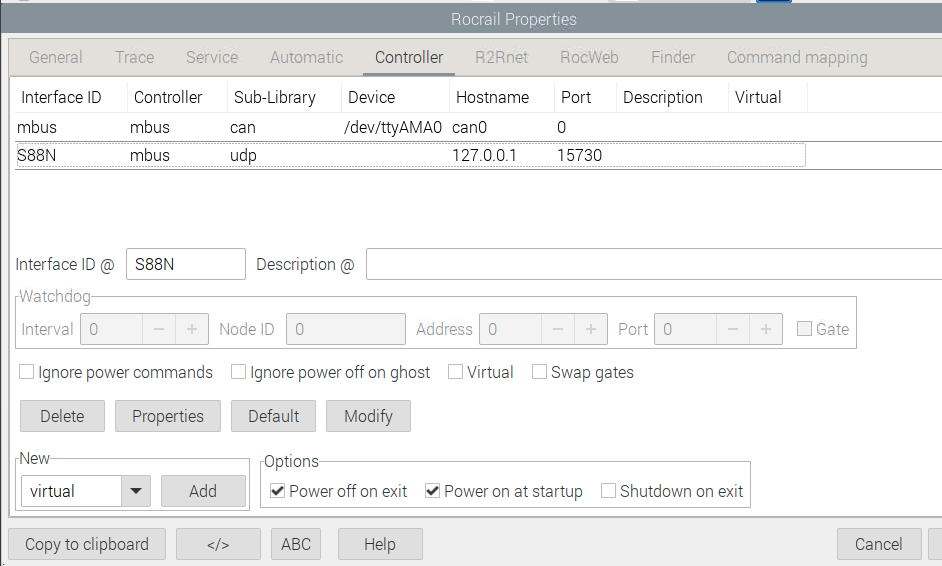
\includegraphics[width=1.00\linewidth]{../figures/rocrailcontrollersettings/rocrail_controller_mbus_S88n.png}
	\caption{General controller settings.}
	\label{rocrail_controller_mbus_S88n}
\end{figure}

\begin{figure}[h!]
	\centering
	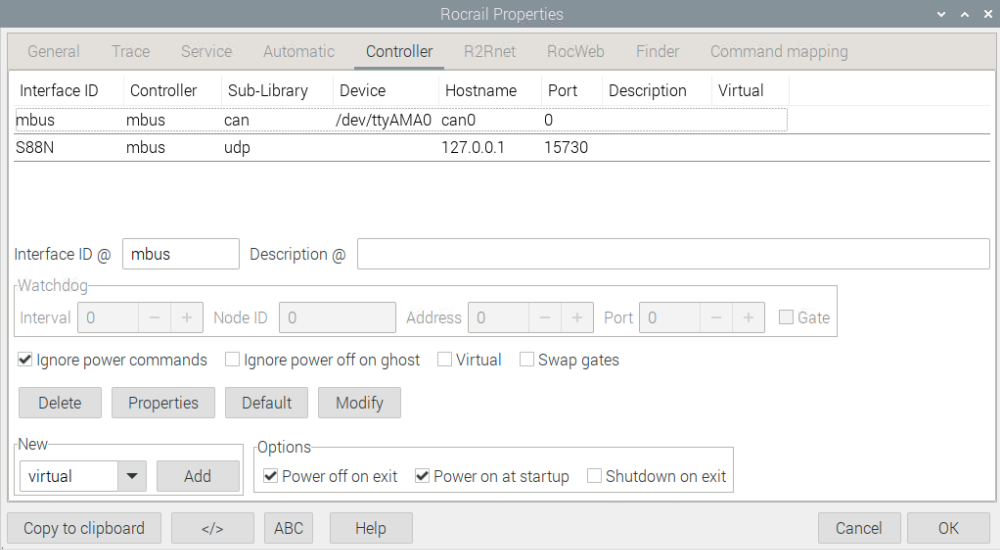
\includegraphics[width=1.00\linewidth]{../figures/rocrailcontrollersettings/generalcontrollersettings.png}
	\caption{General controller settings.}
	\label{fig:generalcontrollersettings}
\end{figure}

\begin{figure}[h!]
	\centering
	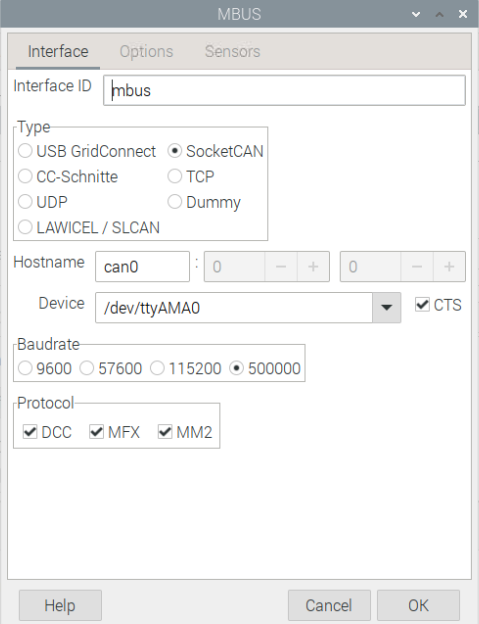
\includegraphics[width=1.00\linewidth]{../figures/rocrailcontrollersettings/mbus_settings_tab1.png}
	\caption{Controller settings mbus-can tab 1.}
	\label{fig:mbus_settings_tab1}
\end{figure}

\begin{figure}[h!]
	\centering
	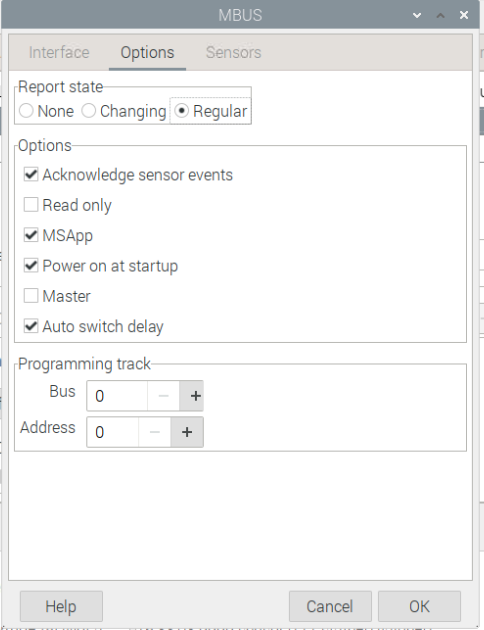
\includegraphics[width=1.00\linewidth]{../figures/rocrailcontrollersettings/mbus_settings_tab2.png}
	\caption{Controller settings mbus-can tab 2.}
	\label{fig:mbus_settings_tab2}
\end{figure}

\begin{figure}[h!]
	\centering
	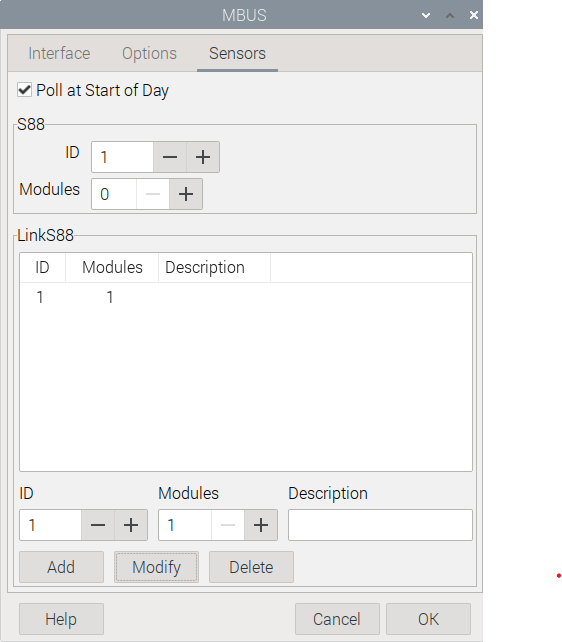
\includegraphics[width=1.00\linewidth]{../figures/rocrailcontrollersettings/mbus_settings_tab3.png}
	\caption{Controller settings mbus-can tab 3.}
	\label{fig:mbus_settings_tab3}
\end{figure}

\begin{figure}[h!]
	\centering
	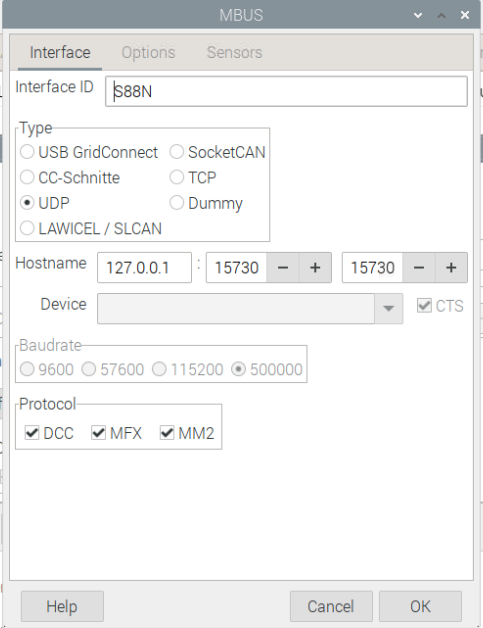
\includegraphics[width=1.00\linewidth]{../figures/rocrailcontrollersettings/S88N_settings_tab1.png}
	\caption{Controller settings mbus-s88 tab 1.}
	\label{fig:S88N_settings_tab1}
\end{figure}

\begin{figure}[h!]
	\centering
	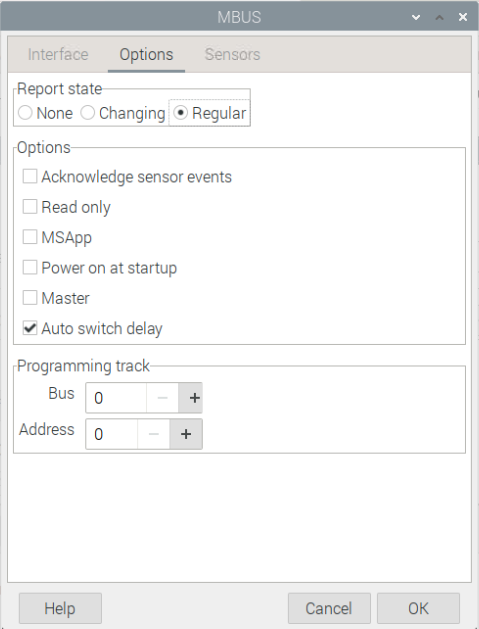
\includegraphics[width=1.00\linewidth]{../figures/rocrailcontrollersettings/S88N_settings_tab2.png}
	\caption{Controller settings mbus-s88 tab 2.}
	\label{fig:S88N_settings_tab2}
\end{figure}

\begin{figure}[h!]
	\centering
	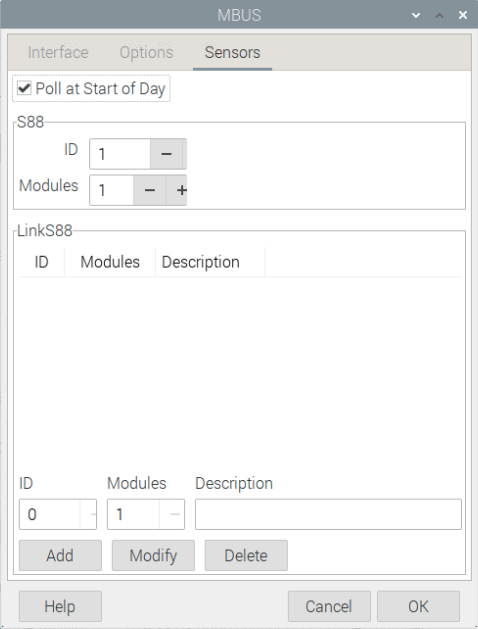
\includegraphics[width=1.00\linewidth]{../figures/rocrailcontrollersettings/S88N_settings_tab3.png}
	\caption{Controller settings mbus-s88 tab 3.}
	\label{fig:S88N_settings_tab3}
\end{figure}
